\documentclass{article}

\usepackage{longtable,relsize,caption,natbib,graphicx}

\title{Technical note: In situ U--Th--He dating by
  \textsuperscript{4}He/\textsuperscript{3}He laser microprobe
  analysis}

\author{Pieter Vermeesch$^1$, Yuntao Tian$^{1,2}$, Jae
  Schwanethal$^{1}$ and Yannick Buret$^3$\\ {London Geochronology
    Centre, Department of Earth Sciences, University College London,
    Gower Street, London WC1E 6BT, United Kingdom}\\ {Guangdong
    Provincial Key Laboratory of Geodynamics and Geohazards, School of
    Earth Sciences and Engineering, Sun Yat-sen University, Guangzhou
    510275, China}\\ {Department of Earth Sciences, Natural History
    Museum, Cromwell Road, London SW7 5BD, United Kingdom} }

\date{}

\begin{document}

\maketitle

\begin{abstract}
  In-situ U-Th-He geochronology is a potentially disruptive technique
  that combines laser ablation inductively coupled plasma mass
  spectrometry (LA-ICP-MS) with laser microprobe noble gas mass
  spectrometry. Despite its potential to revolutionise (detrital)
  thermochronology, in-situ U-Th-He dating is not widely used, due to
  persistent analytical challenges. The main issue is that current
  in-situ U-Th-He dating approaches require that the U, Th and He
  measurements are expressed in units of molar concentration, in
  contrast with conventional methods, which use units of molar
  abundance. Whereas molar abundances can be reliably determined by
  isotope dilution, accurate concentration measurements are not so
  easy to obtain. In the absence of matrix-matched U,Th-concentration
  standards and accurate He-ablation pit measurements, the required
  molar concentration calculations introduce an uncertainty that is
  higher than the conventional method; an uncertainty that is itself
  difficult to accurately quantify. We here present a solution to this
  problem by using proton-induced \textsuperscript{3}He as a proxy for
  ablation pit volume, and by pairing samples with a standard of known
  U-Th-He age. Thus, the U-Th-He age equation can be solved using
  relative rather than absolute concentration measurements.  Pilot
  experiments show that the new method produces accurate results.
  However, it is prone to overdispersion, which is attributed to
  gradients in the proton fluence. These gradients can be measured and
  their effect can be removed by fixing the geometry of the sample and
  the standard during the proton irradiation.
\end{abstract}

\section{Introduction}

Conventional U-Th-He thermochronology is labour intensive, especially
for zircon. It involves (1) identifying suitable crystals under a
binocular microscope; (2) measuring their three-dimensional size to
estimate the fraction of helium lost through $\alpha$-ejection
\citep{farley1996,ketcham2011}; (3) packing the individual crystals
into Pt or Nd `microfurnaces' \citep{house2000}; (4) degassing the
crystals with a laser in ultrahigh vacuum and analysing the released
gas by noble gas mass spectrometry; (5) recovering the degassed grains
from the microfurnaces and dissolving them in hydrofluoric acid with a
Parr vessel; and (6) determining their U and Th content by isotope
dilution ICP-MS (Figure~\ref{fig:method}A).\medskip

In-situ U-Th-He laser microprobe analysis removes steps 2, 3 and 5 of
this procedure, which potentially increases sample throughput whilst
producing U-Pb double-dates as a byproduct. This opens new research
opportunities in detrital geochronology \citep{boyce2006, boyce2009,
  vermeesch2012a, tripathy2013, evans2015, danisik2017}. However,
despite its appeal, the method has still not been widely adopted by
thermochronologists nearly two decades after its initial development
by \citet{boyce2006}. The slow uptake of in-situ U-Th-He dating has
several causes, one of which is accuracy.\medskip

Measuring helium concentration (in units of atoms per unit volume)
requires accurate estimates of ablation pit volume.  Unfortunately,
laser ablation produces irregularly shaped ablation pits in ultra-high
vacuum conditions, making pit volume measurements difficult at best
and inaccurate at worst. The accuracy of the U and Th concentration
measurements cannot be guaranteed either, due to a lack of
matrix-matched concentration standards.\medskip

\citet{vermeesch2012a} proposed a simplified workflow that pairs the
sample with a well characterised reference material of known U-Th-He
age, thereby removing the need for accurate U and Th concentration
measurements. \citet{evans2015} reformulated this `pairwise dating'
approach in terms of a $\kappa$-calibration factor. Given the U/Si,
Th/Si and He/$V$ ratio measurements of a standard of known age $t$,
where $V$ is the ablation pit volume, the U-Th-He age equation can be
written as:
\begin{equation}
  \kappa \left[\frac{He}{V}\right] =
  \left\{
  8 \frac{137.82}{138.82} \left(e^{\lambda_{38}t}-1\right)  +
  \frac{7}{138.82} \left(e^{\lambda_{35}t}-1\right) 
  \right\} \left[\frac{U}{Si}\right] +
  6 \left(e^{\lambda_{32}t}-1\right) \left[\frac{Th}{Si}\right]
  \label{eq:kappa}
\end{equation}

\noindent where $\kappa$ serves a similar purpose as the J-factor in
\textsuperscript{40}Ar/\textsuperscript{39}Ar geochronology
\citep{merrihue1966} or the $\zeta$-calibration factor in fission
track thermochronology \citep{hurford1983}.\medskip

Although this method solves many of the practical difficulties of
in-situ U-Th-He measurements, the need for ablation pit measurements
remains. In its simplest form, the $\kappa$-calibration approach
assumes that the drill rate of the UV laser is the same for the sample
and the standard.  Interferometric pit depth measurements indicate
that this is not the case. For example, \citet{vermeesch2012a}
observed drill rate differences of 15\% even when identical laser
settings were used to analyse different Sri Lanka zircon megacrysts.
These drill rate differences were found to be roughly proporational to
the Si-sensitivity differences measured by LA-ICP-MS, suggesting that
Si can be used as a `drill rate proxy' for the helium
measurements.\medskip

Using Si as a proxy for pit depth works reasonably well for the
samples of \citet{vermeesch2012a}, but is imprecise and only works
when samples and standards are analysed in the same analytical
session, using identical laser settings.\medskip

This paper presents a progress report for a different approach to
pairwise U-Th-He dating, using proton-induced \textsuperscript{3}He as
a proxy for ablation pit volume (Figure~\ref{fig:method}A). When
zircon is irradiated with high energy protons in a particle
accelerator, spallation reactions on Zr, Si and O produce a small but
measurable amount of \textsuperscript{3}He \citep{shuster2004}. If a
sample and co-irradiated reference materials have experienced the same
proton fluence, then Equation~\ref{eq:kappa} can be replaced with:
\begin{equation}
  \kappa \left[\frac{{}^{4}He}{{}^{3}He}\right] =
  \left\{
  8 \frac{137.82}{138.82} \left(e^{\lambda_{38}t}-1\right)  +
  \frac{7}{138.82} \left(e^{\lambda_{35}t}-1\right) 
  \right\} \left[\frac{U}{Si}\right] +
  6 \left(e^{\lambda_{32}t}-1\right) \left[\frac{Th}{Si}\right]
  \label{eq:kappa43}
\end{equation}

The following sections summarise experimental tests of this simple
idea.  These experiments that were carried out between 2014 and 2016
using financial support from the UK's Natural Environment Research
Council (NERC, see Acknowledgments).  The research funding ended, the
research team was dissolved, and research priorities shifted, so that
the results of our work were never published. With this technical
note, we would like to encourage others to continue were we left off,
using the lessons that we have learned.\medskip

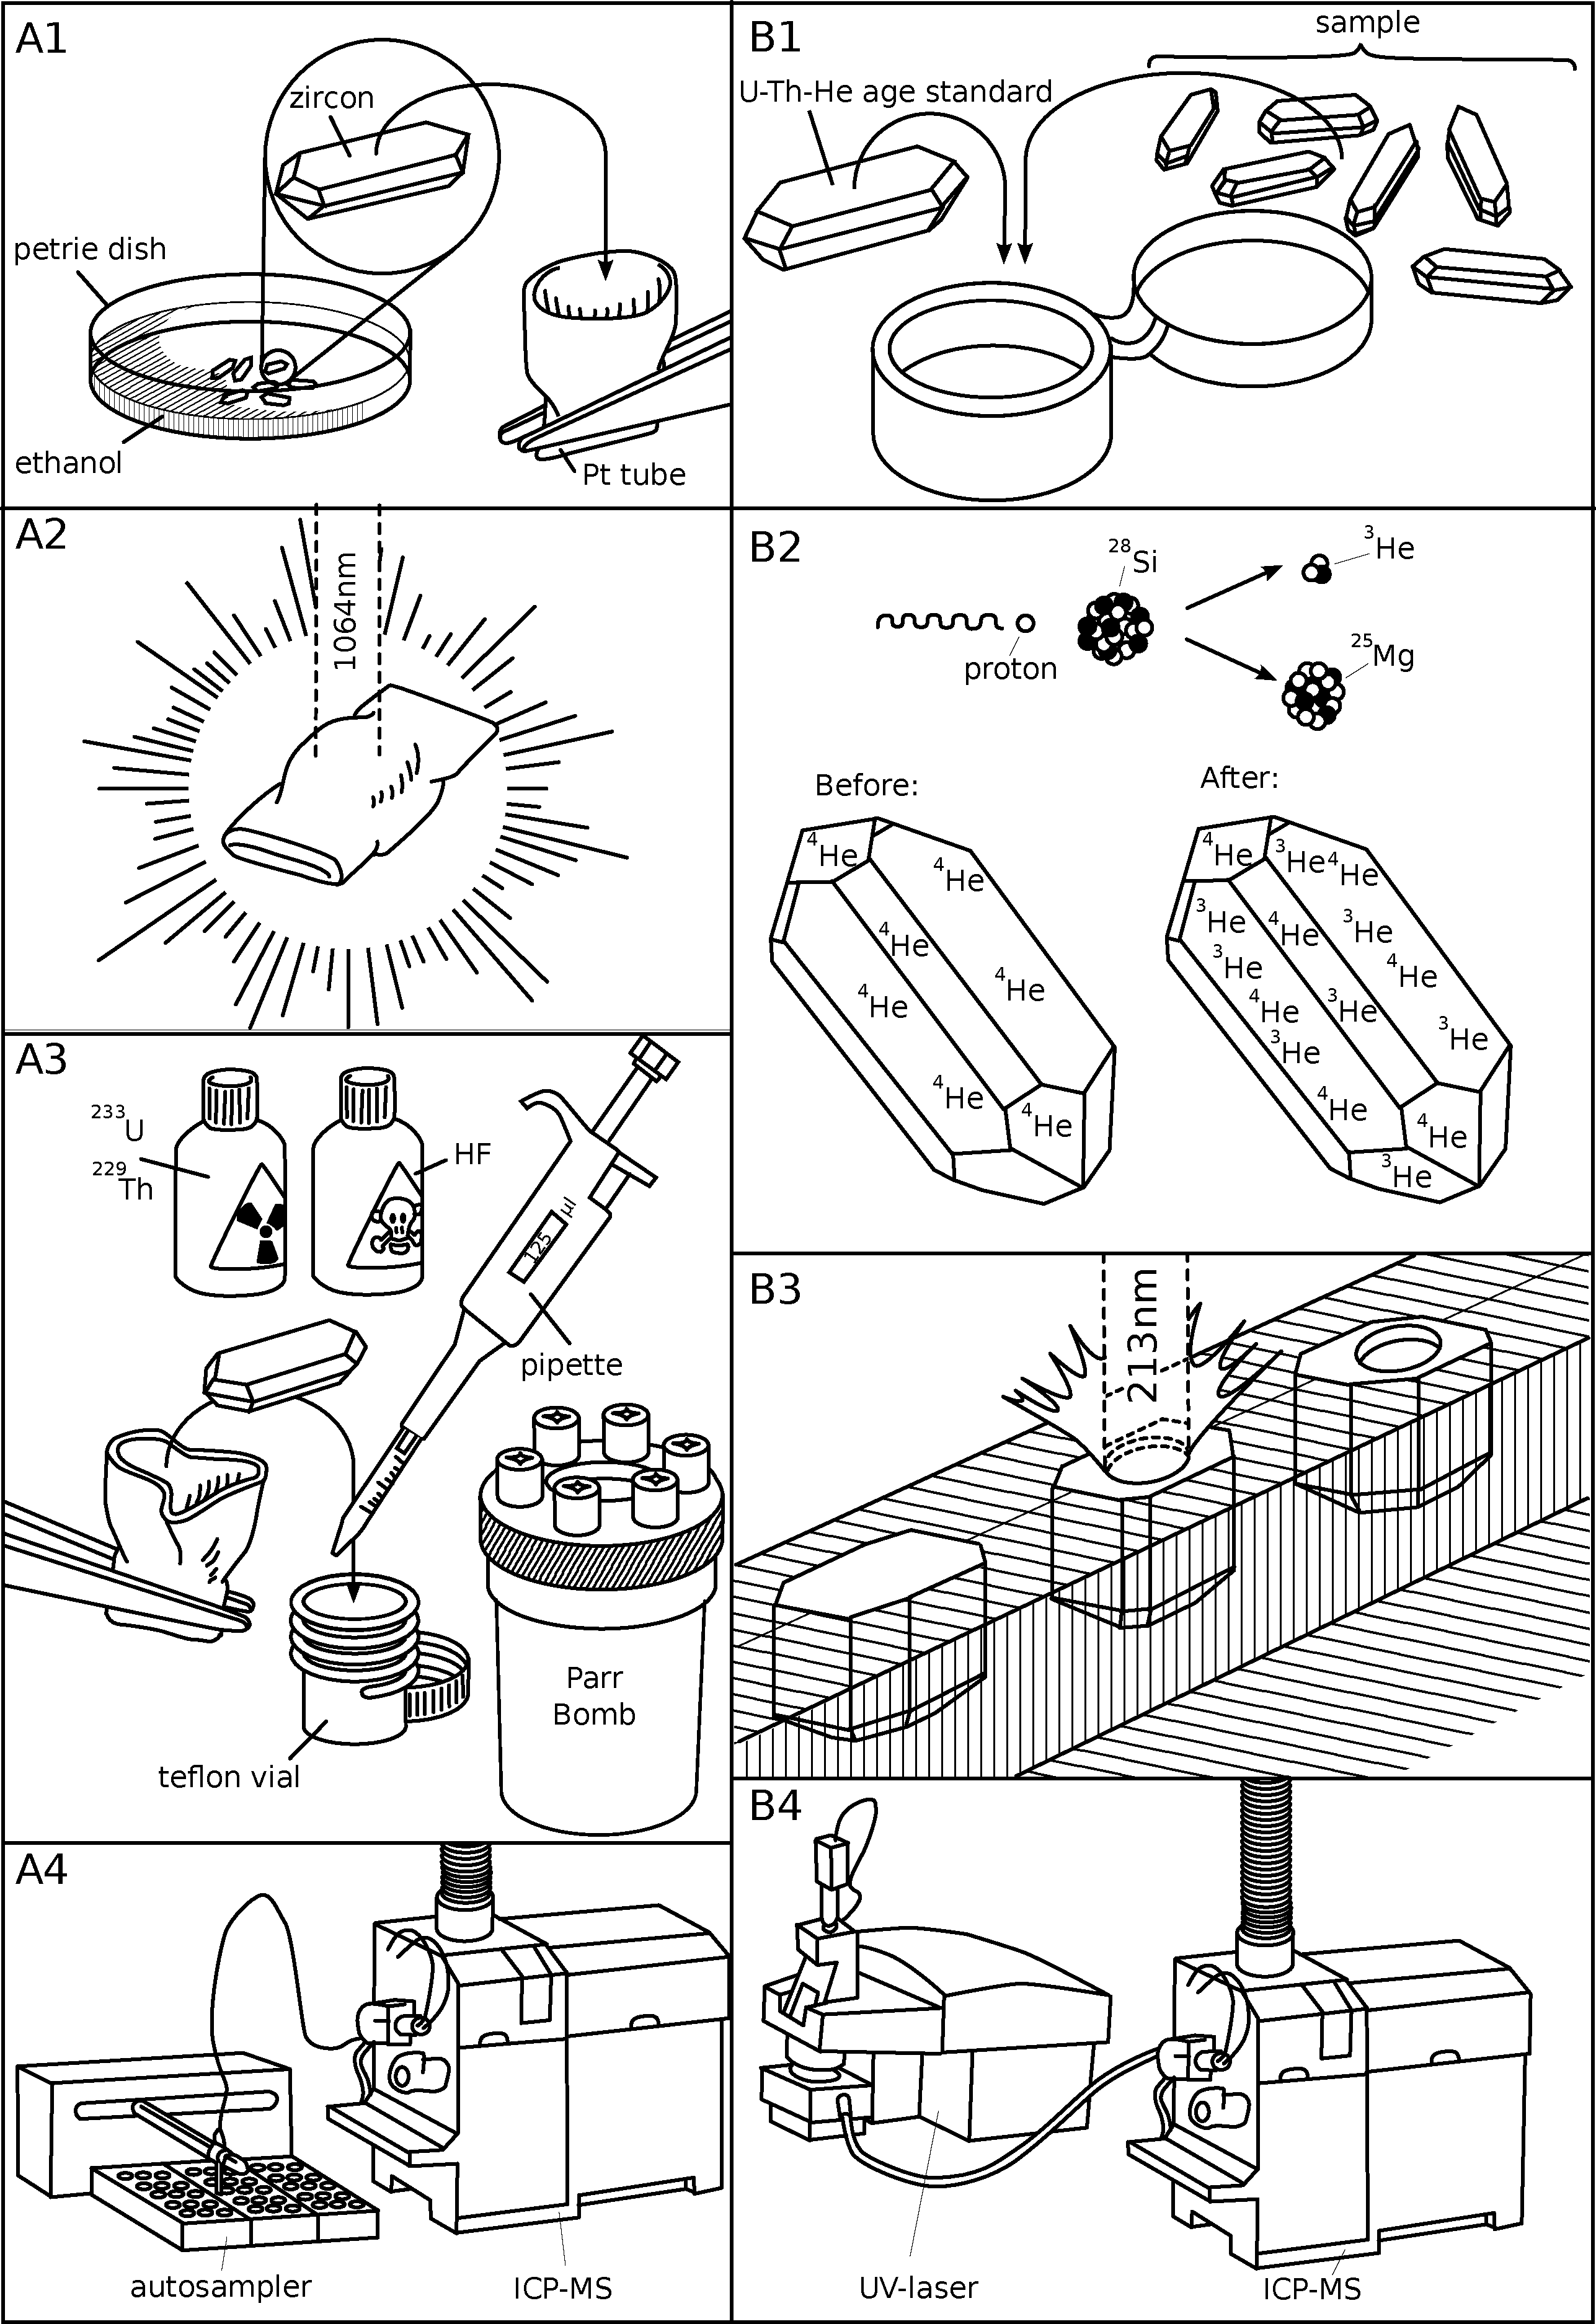
\includegraphics[height=.8\textheight]{method.pdf}
\captionof{figure}{The analytical procedure for conventional U-Th-He
  dating (A) and the new in-situ
  \textsuperscript{4}He/\textsuperscript{3}He laser microprobe method
  (B): A1. grain selection; A2. degassing by laser heating in a Pt
  microfurnace; A3. isotope dilution of U and Th; A4. U and Th
  analysis in solution; B1. packing sample and standard together;
  B2. proton irradiation; B3.
  \textsuperscript{4}He/\textsuperscript{3}He analyses (of vertically
  mounted zircons) by UV laser microprobe noble gas mass spectrometry;
  B4. U and Th analysis by LA-ICP-MS.}
\label{fig:method}

\section{Experimental designs}
\label{sec:design}

We tested three different experimental designs:
\begin{enumerate}
\item{\bf Loose grains:} co-irradiate the sample and the standard in a
  plastic capsule (`rabbit'), without fixing or registering their
  position within the capsule (Section~\ref{sec:loose}).
\item{\bf Vertically mounted grains:} similar to the first design, but
  polishing the grains perpendicular to the c-axis instead of parallel
  to it prior to laser ablation (Section~\ref{sec:vertical}).
\item{\bf Sample-standard `sandwiches':} co-irradiate the sample and the
  standard in a fixed position and attached to each other
  (Section~\ref{sec:sandwich}).
\end{enumerate}

The three experiments were tested sequentially, which means that the
second experimental design was motivated by the outcome of the first
experiment, and the third experiment was motivated by the outcome of
the second experiment. Sections~\ref{sec:loose} and \ref{sec:vertical}
briefly discuss the methods and the results of the first two
experiments.  Section~\ref{sec:sandwich} will describe the
experimental setup of the third experiment. In-depth discussions of
the third method and its results are deferred to
Sections~\ref{sec:methods} and \ref{sec:results}, respectively.

\subsection{Loose grains}\label{sec:loose}

In a first set of experiments, loose grains of Fish Canyon zircon were
packed together with Sri Lanka zircon LGC-1
\citep[476.4$\pm$5.7~Ma,][]{tian2017}. After proton irradiation, the
grains were mounted in teflon, polished, and analysed for U, Th and He
using procedures that are detailed in Section~\ref{sec:methods}. These
experiments produced generally accurate, but highly dispersed results
(Figure~\ref{fig:FCZ}). At first, we attributed this dispersion to
compositional zoning of the Fish Canyon zircons (Figure~\ref{fig:CL}):
because helium is measured in a separate ablation spot from the U and
Th, any difference in actinide concentration between the two spots
causes inaccurate ages.\medskip

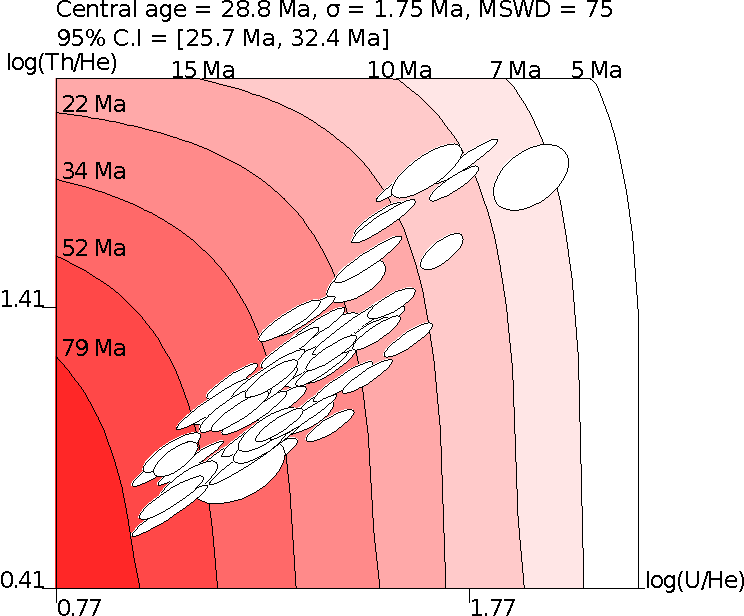
\includegraphics[width=.5\textwidth]{FCZ.pdf} \captionof{figure}{The
  U-Th-He compositions of 61 Fish Canyon zircons (white ellipses)
  follow a bivariate normal U-Th-He distribution in logratio space
  \citep{vermeesch2010a}. The mean composition corresponds to a
  U-Th-He age \citep[the `central age';][]{vermeesch2008a} which is in
  excellent agreement with the known eruption age of the Fish Canyon
  Tuff \citep[28.8Ma, ][]{kuiper2008}. The compositional MSDW of 75
  indicates significant overdispersion with respect to the formal
  analytical precision, likely due to a combination of compositional
  zoning (Figure \ref{fig:CL}) and proton flux gradients. The data for
  this figure are provided as an online supplement.}
\label{fig:FCZ}

\subsection{Vertically mounted grains}\label{sec:vertical}

Because compositional zoning tends to be largely concentric around the
c-axis, we carried out some experiments using vertically mounted Fish
Canyon zircons (Figure~\ref{fig:CL}).  This was achieved by (1)
excavating a series of $100\times{50}\times{50}$~\textmu{m} `trenches'
in sheets of teflon; (2) placing proton-irradiated zircons in them;
(3) covering the grains with a second sheet of teflon; (4) welding the
two sheets together by applying pressure to them on a hot plate at
ca. 210$^\circ$C; (5) polishing the edge of the resulting teflon
`sandwich' until the apexes of the grains were removed; and (6)
placing the teflon sheet upright in a bespoke sample holder. Helium
was measured first, and after repolishing the U and Th were measured
in a second ablation pit located down the c-axis from the first
one. This elaborate procedure slightly reduced the dispersion, but
unfortunately did not remove it.\medskip

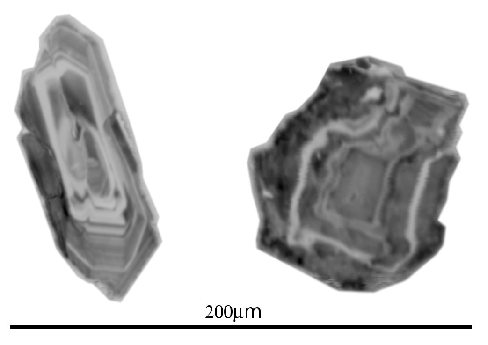
\includegraphics[width=.5\textwidth]{CL.pdf}
\captionof{figure}{Cathodo-luminescence images of horizontally (left)
  and vertically (right) mounted Fish Canyon zircons, exhibiting
  predominantly c-axis concentric compositional zoning.}
\label{fig:CL}

\subsection{Sample-standard `sandwiches'}\label{sec:sandwich}

The previous pair of experiments indicated that, although
compositional zoning may be one factor degrading the accuracy of in-situ
U-Th-He dating, it is not the dominant factor. Closer inspection of
the standards revealed marked differences in
\textsuperscript{4}He/\textsuperscript{3}He ratios within and between
Sri Lanka megacryst shards. These differences suggest the presence of
strong, mm-scale gradients in the proton fluence, despite the efforts
taken to change the orientation of the samples during the
irradiation.\medskip

To investigate this phenomenon and potentially fix it, we developed a
third experimental design, in which the standard and sample are
polished prior to irradiation and glued together along their polishing
surfaces. This arrangement serves a dual purpose. First, it ensures
that each point in the sample receives exactly the same proton dose as
its counterpart in the standard. Second, by attaching the sample to
the standard, any spallogenic \textsuperscript{3}He that passes
through the polishing surface of the sample is injected into the
standad and \emph{vice versa}. This reduces potential geometric
complications that may arise when comparing different sized
crystals. We tested this approach using compositionally homogeneous
GJ-1 \citep{jackson2004} as a sample, to avoid the confounding effect
of textural complexity in FC zircon. The results of these experiments
are described and discussed in the remainder of this paper.

\section{Analytical methods and data processing}
\label{sec:methods}

The sample-standard sandwiches were packed together in HDPE vials
(Posthumus Plastics capsule type H and snapcap type E) and
proton-irradiated at the Massachussetts General Hospital using
procedures outlined by \citet{shuster2004}. Samples were attached to
standards using super glue, and were detached after irradiation by
dissolution of the glue with acetone in an ultrasonic bath. The
detached crystals were rinsed in de-ionised water and mounted in
indium. Photographically identified contact points were used to match
any location in the sample with its `mirror image' in the
standard.\medskip

Helium was released from the zircon grains by ablation with a UP-213
frequency-quintupled Nd-YAG laser in a small (5~cm diameter) ablation
cell with sapphire window. Typical spot sizes were 90~\textmu{m} in
diameter, with ablation occurring at 20~Hz for
30~seconds. \textsuperscript{4}He was measured on a Faraday detector
and \textsuperscript{3}He on a secondary electron multiplier (SEM) in
peaking hopping mode (using either six or twenty 85-second cycles) on
a Nu Instruments Noblesse sector field noble gas mass spectrometer at
University College London. The extraction line of this instrument is
described by \citet{schwanethal2015}, as is the procedure to minimise
the \textsuperscript{12}C\textsuperscript{3+} interference on
\textsuperscript{4}He.\medskip

The \textsuperscript{4}He/\textsuperscript{3}He ratio was obtained by
linear regression of the \textsuperscript{4}He signals and
\textsuperscript{3}He to `time zero', which corresponds to the time
when the cleaned gas was introduced into the ionisation volume of the
mass spectrometer.  The resulting values have units of mV/Hz. Note
that these units vanish from the age equation after encapsulation in
the $\kappa$-calibration constant (Equation~\ref{eq:kappa}). Thus, our
method does not require the sensitivity of the Faraday and SEM
detectors to be inter-calibrated.\medskip

The U and Th content of the samples was analysed by LA-ICP-MS at the
Natural History Museum, using an Agilent 8900 instrument that was
coupled with a Teledyne Cetac Iridia laser. This setup is optimised
for raster imaging applications. Each grain was mapped using a
${10}\times{10}$~\textmu{m} square spot with an energy density of
2.5~J/cm\textsuperscript{2}, a repetition rate of 400~Hz and a scan
speed of 400~\textmu{m/s}. ICP-MS measurements used dwell times of
2.5~ms for all measured isotopes (\textsuperscript{29}Si,
\textsuperscript{206}Pb, \textsuperscript{232}Th and
\textsuperscript{238}U). NIST SRM610 was used as a concentration
standard and 91500 zircon as a secondary reference material. Data
reduction was done with Teledyne Cetac's HDIP software. This method
allowed us to create U,Th-maps with 10~\textmu{m} horizontal
resolution. These detailed maps allowed us to (1) detect any
compositional zoning in the sample and standard, and (2) interpolate
the U,Th-concentrations to the locations of the helium analysis spots.
\medskip

This analytical protocol produces the following data files:

\begin{enumerate}
\item A table with the coordinates ($x, y$) of the helium ablation
  spots, the corresponding blank-corrected
  \textsuperscript{4}He/\textsuperscript{3}He measurements, and their
  standard errors, for both halves of the sample-standard sandwich.
  The coordinates can be expressed in LA-ICP-MS laser stage
  coordinates by identifying the helium ablation spots in the
  U,Th-map.
\item Two grids of U and Th concentration measurements or,
  equivalently, U/Si and Th/Si ratio measurements.
\item A table of fiducial points, recording the positions of at least
  three matching locations in the sample and the standard, recorded in
  LA-ICP-MS laser stage coordinates.
\end{enumerate}

Given these three pieces of information, the U-Th-He ages are
calculated as follows:

\begin{enumerate}
\item Map the coordinates of the standard onto those of the sample by
  Procrustes analysis, using the fiducial points
  (Figure~\ref{fig:results}a-b).
\item Interpolate the U and Th concentration (or U/Si and Th/Si ratio)
  measurements to the locations of the
  \textsuperscript{4}He/\textsuperscript{3}He measurements
  (Figure~\ref{fig:results}c).
\item Calculate the $\kappa$-calibration constant for each helium
  ablation spot in the standard, given its known age and U, Th and
  \textsuperscript{4}He/\textsuperscript{3}He measurement.
\item Interpolate the $\kappa$-values of the standard to the locations
  of the helium measurements in the sample.
\item Combine the $\kappa$ parameter with the
  \textsuperscript{4}He/\textsuperscript{3}He, U and Th measurements
  of the sample to calculate the U-Th-He age
  (Figure~\ref{fig:results}.d-e).
\end{enumerate}

\section{Results}
\label{sec:results}

Inspection of the analytical results for two standard-sample pairs
(Tables~\ref{tab:results1} and \ref{tab:results2}) reveals a number of
patterns. First, the \textsuperscript{4}He/\textsuperscript{3}He
ratios vary significantly between different shards of LGC-1 and
GJ-1. They are, on average, 25\% higher for the first pair than for
the second pair. In contrast, the U and Th concentrations of the two
pairs of shards are nearly identical. This discrepancy between the two
sets of measurements can only have one cause, namely the presence of
significant gradients in the proton fluence received by different
parts of the `rabbit'. These gradients are reflected in the
$\kappa$-values, which vary in tandem with the
\textsuperscript{4}He/\textsuperscript{3}He measurements.\medskip

Whilst the $\kappa$-values vary by a factor of two between the pairs,
smaller gradients are visible within them. For example, pair~1
exhibits a $\sim$15\% difference in $\kappa$-values over a distance of
$\sim$500~\textmu{m}. Fitting an interpolation surface to these values
undoes the effect of the proton gradient and produces more accurate
ages (Figure~\ref{fig:results}.c).\medskip

For pair~1, the in-situ U-Th-He ages range from 420 to 520~Ma, with a
central age of 453$\pm$8~Ma, which is in good agreement with
conventional U-Th-He ages of GJ-1 (456$\pm$13~Ma,
Table~\ref{tab:conventional}). The second pair yields equally accurate
ages, ranging from 420 to 500~Ma with a central value of
457$\pm$24~Ma. The compositional MSWDs \citep[as defined
  by][]{vermeesch2010a} of 1.5 for the first pair
(Figure~\ref{fig:results}e), and 2.3 for the second pair indicate that
overdispersion is minor.  Thus, the sandwich technique appears to have
successfully removed the proton fluence gradient.

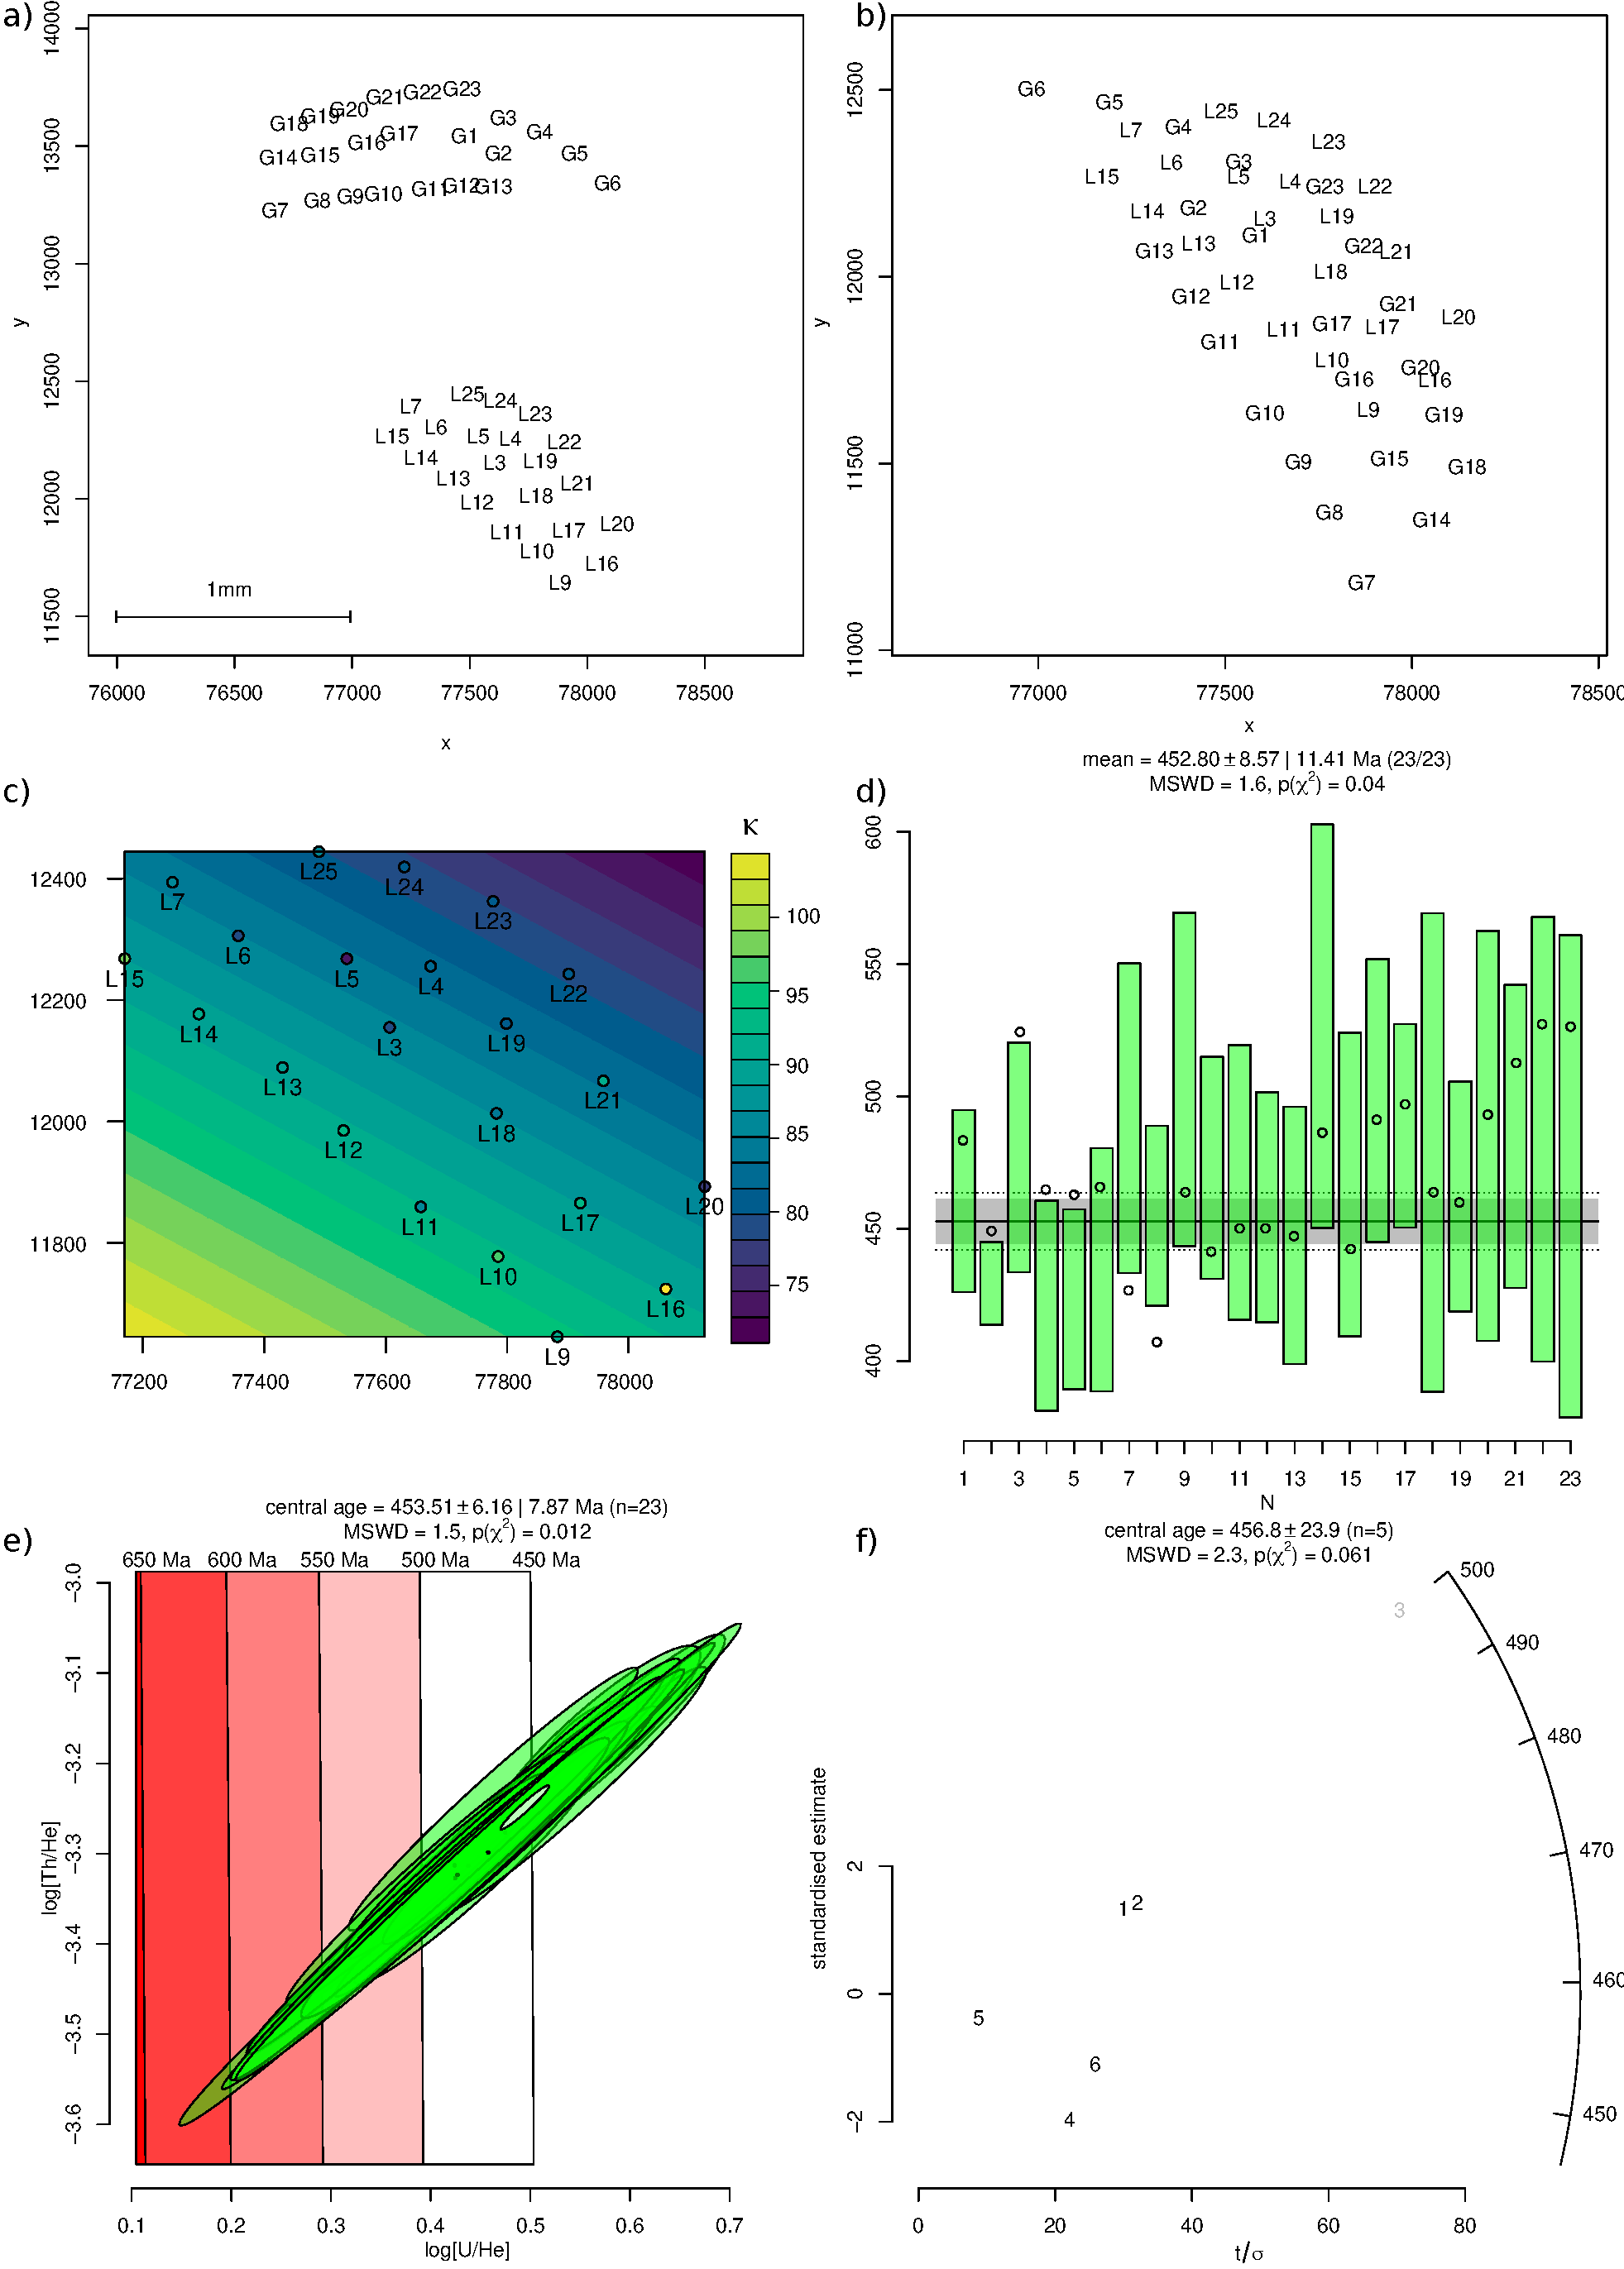
\includegraphics[height=.9\textheight]{results2.pdf}
\captionof{figure}{a) stage coordinates of the helium measurements for
  the standard (`L' is short for `LGC-1') and sample (`G' is short for
  `GJ-1') of the first sample-standard pair; b)
  Procrustes-transformation of the coordinates in the previous panel;
  c) linear interpolation surface of the $\kappa$-values for LGC-1; d)
  U-Th-He age estimates for the first sample-standard pair
  (conventional age = ${456.0}\pm{12.7}$~Ma), with open circles
  representing the ages calculated using a uniform $\kappa$-value; e)
  U-Th-He compositions for the first sample-standard pair; f) radial
  plot with the U-Th-He age estimates for the second sample-standard
  pair, with the third aliquot omitted as an outlier.\medskip}
\label{fig:results}

\captionof{table}{Analytical results for the first pair of LGC-1 and
  GJ-1 shards. Row names represent helium laser ablation spots
  (LGC1-1-n and GJ1-1-n where `n' is a number) and fiducial marks
  (LGC1-1-X and GJ1-1-X where `X' is a letter). Columns $x$ and $y$
  represent the raw LA-ICP-MS stage coordinates (in microns) of the
  helium spots; $x'$ and $y'$ are the coordinates after Procrustes
  transformation; \textsuperscript{4}He/\textsuperscript{3}He and
  s[\textsuperscript{4}He/\textsuperscript{3}He] have units of mV/Hz;
  \textsuperscript{3}He has units of Hz; U, s[U], Th and s[Th] have
  units of ppm; $\kappa$ and s[$\kappa$] have units of Hz/mV; and t
  and s[t] are in Ma.}
\label{tab:results1}
\relsize{-0.5}
\addtolength\tabcolsep{-0.05em}
\begin{longtable*}{@{}l@{~~}l@{~~}l@{~~}l@{~~}l@{~~}l@{~~}l@{~~}l@{~~}l@{~~}l@{~~}l@{~~}l@{~~}l@{~~}l@{~~}l@{~~}l@{}}
&$x$&$y$&$x'$&$y'$&\textsuperscript{4}He/\textsuperscript{3}He&s[\textsuperscript{4}He/\textsuperscript{3}He]&\textsuperscript{3}He&U&s[U]&Th&s[Th]&$\kappa$&s[$\kappa$]&$t$&$s[t]$\\ \hline
\endhead
LGC1-1-A&77776&12719&&&&&&&&&&&&&\\
LGC1-1-B&78317&11724&&&&&&&&&&&&&\\
LGC1-1-C&76709&12592&&&&&&&&&&&&&\\
LGC1-1-3&77606&12155&77606&12155&3.59&0.118&12&310&2&570&3.5&77.9&2.61&476.4&5.7\\
LGC1-1-4&77674&12256&77674&12256&3.42&0.224&21&310&2&570&3.8&82.2&5.41&476.4&5.7\\
LGC1-1-5&77536&12268&77536&12268&3.83&0.0908&18&310&2.2&570&3.7&73.5&1.82&476.4&5.7\\
LGC1-1-6&77357&12306&77357&12306&3.58&0.213&21&310&2.1&570&3.6&78.4&4.68&476.4&5.7\\
LGC1-1-7&77249&12394&77249&12394&3.37&0.0965&22&310&1.8&570&3.2&84.5&2.46&476.4&5.7\\
LGC1-1-9&77883&11645&77883&11645&3.25&0.125&21&320&2&600&4&89.9&3.52&476.4&5.7\\
LGC1-1-10&77785&11777&77785&11777&3.05&0.129&13&320&2&590&4.4&95.4&4.09&476.4&5.7\\
LGC1-1-11&77658&11859&77658&11859&3.4&0.189&12&310&1.9&590&3.9&84.5&4.73&476.4&5.7\\
LGC1-1-12&77530&11985&77530&11985&3.06&0.0805&13&310&2.1&580&3.9&91.8&2.5&476.4&5.7\\
LGC1-1-13&77430&12089&77430&12089&3.17&0.154&13&310&2.3&570&4&88.8&4.36&476.4&5.7\\
LGC1-1-14&77292&12177&77292&12177&3.12&0.0641&13&310&1.9&580&3.3&90.9&1.94&476.4&5.7\\
LGC1-1-15&77170&12268&77170&12268&2.94&0.0989&9&310&1.8&580&3.2&96.3&3.29&476.4&5.7\\
LGC1-1-16&78061&11724&78061&11724&2.82&0.0714&13&320&2.1&600&4.2&104&2.73&476.4&5.7\\
LGC1-1-17&77921&11865&77921&11865&3.18&0.166&12&320&2.2&590&4.2&91.2&4.81&476.4&5.7\\
LGC1-1-18&77782&12013&77782&12013&3.39&0.195&11&310&2&580&3.3&84.3&4.88&476.4&5.7\\
LGC1-1-19&77799&12161&77799&12161&3.57&0.248&10&310&2.6&590&4.6&80.5&5.63&476.4&5.7\\
LGC1-1-20&78126&11893&78126&11893&3.9&0.311&9&330&2.3&610&5&76.8&6.13&476.4&5.7\\
LGC1-1-21&77959&12067&77959&12067&3.27&0.148&10&320&2.1&590&3.9&89.6&4.1&476.4&5.7\\
LGC1-1-22&77902&12243&77902&12243&3.66&0.218&9.4&320&2&590&4.1&79.5&4.77&476.4&5.7\\
LGC1-1-23&77777&12363&77777&12363&3.6&0.147&8.6&320&2&580&3.2&80.7&3.32&476.4&5.7\\
LGC1-1-24&77631&12419&77631&12419&3.62&0.231&8.7&320&1.9&590&3.3&80.1&5.13&476.4&5.7\\
LGC1-1-25&77490&12444&77490&12444&3.39&0.181&8.9&320&1.8&580&3.5&85.5&4.6&476.4&5.7\\
GJ1-1-A&77744&14021&&&&&&&&&&&&&\\
GJ1-1-B&76830&13858&&&&&&&&&&&&&\\
GJ1-1-C&78323&13183&&&&&&&&&&&&&\\
GJ1-1-1&77479&13545&77582&12112&1.94&0.0731&17&270&2.4&6.3&0.059&86.9&0.871&460&18\\
GJ1-1-2&77623&13469&77416&12185&1.8&0.0218&17&270&2.5&6.3&0.072&87.3&1.04&430&8\\
GJ1-1-3&77642&13623&77537&12309&2.1&0.0955&15&270&2.5&6.1&0.06&82.6&1.19&480&22\\
GJ1-1-4&77797&13561&77375&12402&1.86&0.0854&20&270&3.1&6.2&0.066&82.5&1.38&420&20\\
GJ1-1-5&77946&13469&77190&12468&1.86&0.0647&20&270&3.9&6.3&0.079&83.3&1.7&420&17\\
GJ1-1-6&78087&13344&76982&12504&1.93&0.0951&19&280&2.5&6.3&0.069&85.2&2.19&430&23\\
GJ1-1-7&76672&13227&77866&11182&1.7&0.0831&14&270&1.9&6.4&0.047&106&4.3&490&30\\
GJ1-1-8&76852&13271&77779&11371&1.64&0.03&11&280&2.2&6.4&0.053&103&3.55&450&17\\
GJ1-1-9&76993&13289&77697&11506&1.88&0.111&12&280&1.8&6.4&0.048&100&3.05&510&32\\
GJ1-1-10&77133&13298&77606&11636&1.81&0.0696&13&280&2.2&6.4&0.057&98.4&2.63&470&21\\
GJ1-1-11&77333&13321&77487&11827&1.76&0.0962&13&270&2.3&6.4&0.064&95.2&2.05&470&26\\
GJ1-1-12&77462&13333&77408&11949&1.86&0.086&10&280&2.6&6.5&0.067&93.3&1.76&460&22\\
GJ1-1-13&77600&13331&77310&12069&1.88&0.102&12&290&2.5&6.7&0.07&91.6&1.65&450&25\\
GJ1-1-14&76686&13451&78053&11351&1.95&0.137&9.9&270&2.2&6.2&0.048&99.5&3.26&530&39\\
GJ1-1-15&76863&13464&77940&11515&1.79&0.107&10&280&2.1&6.3&0.05&96.9&2.64&470&29\\
GJ1-1-16&77063&13515&77846&11726&2&0.107&8.8&280&2.5&6.5&0.052&93&1.83&500&27\\
GJ1-1-17&77201&13556&77786&11875&2.06&0.0792&8.3&280&2.5&6.6&0.056&90.1&1.33&490&20\\
GJ1-1-18&76731&13596&78149&11491&1.88&0.182&8.7&280&1.9&6.3&0.051&94.7&2.7&480&46\\
GJ1-1-19&76863&13630&78086&11630&1.86&0.0807&8.7&280&2.2&6.3&0.059&92.1&2.23&460&22\\
GJ1-1-20&76987&13656&78023&11757&2.05&0.169&7.8&280&2.2&6.5&0.055&89.8&1.85&490&40\\
GJ1-1-21&77139&13709&77964&11928&2.08&0.125&7.3&280&2.6&6.3&0.07&86.4&1.55&480&29\\
GJ1-1-22&77299&13731&77871&12083&2.11&0.192&4.4&270&2.3&6.2&0.054&83.8&1.42&480&43\\
GJ1-1-23&77468&13746&77767&12242&2.13&0.216&5.8&270&2.4&6.2&0.054&81.2&1.53&470&46\\
\end{longtable*}
\addtolength\tabcolsep{+0.05em}
\relsize{+0.5}


\captionof{table}{Analytical results for the second pair of LGC-1 and
  GJ-1 shards. Row and column names follow the same convention as
  Table~\ref{tab:results1}. The large uncertainties of the
  $\kappa$-calibration constant of the sample are caused by the
  arrangement of the laser spots in two poorly aligned 1D arrays.
  These uncertainties have been omitted from the error propagation.}
\label{tab:results2}
\relsize{-0.5}
\addtolength\tabcolsep{-0.05em}
\begin{longtable*}{@{}l@{~~}l@{~~}l@{~~}l@{~~}l@{~~}l@{~~}l@{~~}l@{~~}l@{~~}l@{~~}l@{~~}l@{~~}l@{~~}l@{~~}l@{~~}l@{}}
&$x$&$y$&$x'$&$y'$&\textsuperscript{4}He/\textsuperscript{3}He&s[\textsuperscript{4}He/\textsuperscript{3}He]&\textsuperscript{3}He&U&s[U]&Th&s[Th]&$\kappa$&s[$\kappa$]&$t$&$s[t]$\\ \hline
\endhead
LGC1-2-A&83616&13266&&&&&&&&&&&&&\\
LGC1-2-B&83949&13588&&&&&&&&&&&&&\\
LGC1-2-C&83511&14479&&&&&&&&&&&&&\\
LGC1-2-D&82563&15181&&&&&&&&&&&&&\\
LGC1-2-3&83547&13646&83547&13646&4.1&0.118&12&310&1.8&590&3.2&69.3&(2.04)&476.4&5.7\\
LGC1-2-4&83489&13744&83489&13744&4.41&0.254&21&300&2.1&570&3.6&62.5&(3.62)&476.4&5.7\\
LGC1-2-5&83427&13835&83427&13835&3.91&0.166&14&300&2&580&3.5&71.1&(3.05)&476.4&5.7\\
LGC1-2-6&83401&13950&83401&13950&4.36&0.16&11&310&1.8&590&3.3&64.7&(2.41)&476.4&5.7\\
LGC1-2-7&83322&14035&83322&14035&4.63&0.162&9.6&300&2.6&580&5&60.3&(2.17)&476.4&5.7\\
LGC1-2-8&83276&14121&83276&14121&4.27&0.15&8.6&310&2.3&580&4.7&65.7&(2.37)&476.4&5.7\\
GJ1-2-A&83479&15581&&&&&&&&&&&&&\\
GJ1-2-B&83617&15974&&&&&&&&&&&&&\\
GJ1-2-C&84275&15383&&&&&&&&&&&&&\\
GJ1-2-D&84485&14460&&&&&&&&&&&&&\\
GJ1-2-1&83746&15498&83507&13803&2.28&0.0785&20&230&2.4&5.8&0.057&65.3&(8.01)&480&16\\
GJ1-2-2&83850&15407&83436&13966&2.42&0.0725&19&230&2.7&5.8&0.069&62.7&(11.2)&480&15\\
GJ1-2-3&83939&15324&83369&14107&2.67&0.032&7.6&240&2.1&5.9&0.048&60.6&(13.4)&500&7.1\\
GJ1-2-4&84062&15311&83401&14264&2.56&0.119&8.6&250&2.3&6.1&0.053&55.1&(32.8)&420&19\\
GJ1-2-5&84102&15218&83302&14349&2.67&0.317&9.4&250&2.3&6.1&0.064&55.5&(24.7)&440&50\\
GJ1-2-6&84151&15103&83180&14455&2.7&0.106&9&250&2.2&6.1&0.048&56.1&(15.4)&440&17\\
\end{longtable*}
\addtolength\tabcolsep{+0.05em}
\relsize{+0.5}

 
\begin{table}[!ht]
  \caption{Conventional U--Th--He data for GJ-1 zircon.}
  \begin{tabular}{ccccccc}
    aliquot & U [pmol] & Th [pmol] & He [pmol] & t [Ma] & s[t] \\ \hline
    1 & 6.550 & 0.437 & 4.105 & 461.0 & 19.0 \\
    2 & 24.057 & 0.980 & 14.709 & 449.8 & 18.0 \\
    3 & 22.283 & 0.922 & 13.626 & 449.8 & 18.0 \\
    4 & 11.028 & 0.822 & 6.839& 452.8 & 18.1 \\
    5 & 6.934 & 0.197 & 4.356 & 462.9 & 18.0 \\
    6 & 2.940 & 0.069 & 1.856 & 465.5 & 19.0 \\
    7 & 6.028 & 0.132 & 3.752 & 459.4 & 19.0 \\
    8 & 2.799 & 0.042 & 1.696 & 448.3 & 18.2
  \end{tabular}
  \label{tab:conventional}
\end{table}

\section{Discussion}
\label{sec:discussion}

The experiments reported in this paper are, in several ways, a best
case scenario.  They compared two zircon megacrysts of similar age
that are compositionally homogeneous. In fact, GJ-1 is so well behaved
that it could also be used as a reference material for in-situ U-Th-He
dating. It remains to be seen if the method is equally successful when
applied to more representative examples, in which zircons are small
and compositionally zoned.\medskip

The $\kappa$-calibration method hinges on the availability of these
well characterised reference materials. They need to be available in
sufficient quantities to be included with every proton irradiation.
In this regard the method is similar to the
\textsuperscript{40}Ar/\textsuperscript{39}Ar method. In this study,
we have used LGC-1 as a reference material. However, the supply of
this standard is limited. As mentioned in the previous paragraph, GJ-1
is also suitable as a reference material. Unfortunately it, too, is
obtained from a single cm-sized crystal. It would be useful to
identify a more abundant alternative. \citet{tian2017} outline a
workflow for doing so.\medskip

The most important requirement for an age standard is the absence of a
distinct diffusion gradient. This, in turn, requires that it has
resided at surface conditions for most of its existence after initial
rapid cooling.  Several Sri Lanka zircons appear to meet this
requirement.\medskip

The sandwich method requires megacrystic standards, which are large
enough to cover the entire sample (Figure~\ref{fig:pairing}a). Finer
grained standards would need a different analytical design. One option
would be to mount the polished sample and standard grains together
prior to irradiation, and attach them both to a cover slip made of
glass or zirconia (Figure~\ref{fig:pairing}b). Assuming that the
proton beam intensity varies smoothly within the irradiation stack,
the $\kappa$-calibration constant could then be obtained by
interpolation between the different aliquots of the standard.\medskip

The in-situ \textsuperscript{4}He/\textsuperscript{3}He method
requires a sector field noble gas mass spectrometer, unlike the
quadrupole instruments that dominate the field of U-Th-He
thermochronology today. Combined with the need for proton irradation,
this makes the new method more expensive than the conventional
approach. Nevertheless, we would argue that our approach merits
further investigation, because it opens the door to new avenues of
research.\medskip

For example, by repeatedly alternating
\textsuperscript{4}He/\textsuperscript{3}He and U, Th measurements in
a raster pattern on the same grain, it would be possible to create
U-Th-He depth profiles, or even reconstruct a 3-dimensional U-Th-He
image by ablating a way the entire crystal, one layer at a time. This
would allow the reconstruction of diffusion profiles and thermal
history models equivalent to those obtained by
\textsuperscript{4}He/\textsuperscript{3}He step-heating experiments
\citep{tripathy2015}, but without the need to assume compositional
homogeneity.\medskip

Although we used a high end raster lasering system for our LA-ICP-MS
experiments, U and Th concentrations could also be determined as
individual spot measurements. We measured He first, and U,Th later.
However, it should also be possible to reverse this order.  The
collateral heating effect of UV laser ablation have been shown to be
negligible \citep[in apatite;][]{vansoest2011}, so that virtually no
helium is lost during the U and Th measurements. Thus, it should be
possible to measure U and Th first, as individual spot measurements,
and revisit the same spots during subsequent helium extraction. This
would remove step~2 (U,Th-interpolation) of the data reduction
procedure outlined in Section~\ref{sec:methods}.\medskip

Although the pilot experiments were time consuming, the proton
irradiation approach offers the potential for high sample throughput.
In contrast with conventional U-Th-He analysis, in which each
individual zircon crystal must be hand picked and packaged, in-situ
analysis allows multiple zircons to be mounted together. Laser
ablation is more easily automated (by pre-programming laser stage
coordinates) than laser microfurnace heating (which additionally
requires automated optical pyrometry). Data processing of in-situ
U-Th-\textsuperscript{4}He/\textsuperscript{3}He dating is also
significantly easier than for other analytical approaches. It does not
require spike calibration or ablation pit depth measurements. The data
can be concisely summarised in simple tables (e.g.,
Table~\ref{tab:results1}).\medskip

If the promise of increased throughput is fulfilled, then arguably the
most important application for in-situ
U-Th-\textsuperscript{4}He/\textsuperscript{3}He thermochronology is
in U-Th-He/Pb double dating. Currently, detrital zircon U-Pb
geochronology is the method of choice for sedimentary provenance
analysis. However, in many places around the world, it is found that
zircon U-Pb age spectra exhibit insufficient variability to resolve
sedimentary provenance. For example, in the Sahara desert, essentially
the same age spectra are found from Mauritania to Egypt
\citep{pastore2021}. The likely reason for this remarkable uniformity
is recycling of older sandstones.  Double dating of detrital zircons
offers a potential solution to this problem: the U/Pb age would be
controlled by the `protosource' of the sediment, whereas the U-Th-He
age would be more sensitive to secondary resetting. U-Th-He/Pb double
dating is very time consuming using traditional methods, which require
separate analysis for U-Pb and U-Th-He analysis
\citep{reiners2005}. In contrast, in-situ methods produce U-Pb dates
as a byproduct of the U,Th-measurements, so double-dates are generated
`for free'.

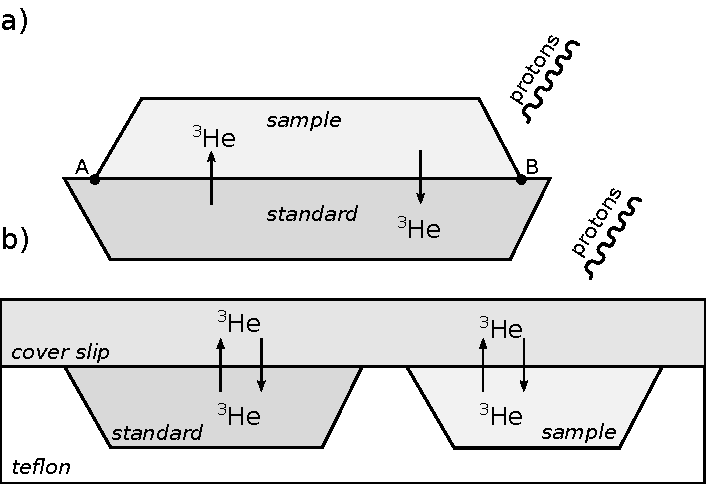
\includegraphics[width=.4\textwidth]{pairing.pdf}
\captionof{figure}{Two ways to quantify and correct proton gradients:
  a) the sample-standard `sandwich' method used in this work, where A
  and B are fiducial points; and b) mounting the sample and the
  standard in teflon and attaching them to a cover slip made of glass
  or zirconia. In both designs, the irradiation geometry is fixed so
  that it is possible to quantify proton flux gradients, and ejection
  of spallogenic \textsuperscript{3}He is balanced by injection from
  neigbouring sources.}
\label{fig:pairing}

\section{Conclusions}

This paper introduced a novel method for in-situ U-Th-He geochronology
that removes the need for absolute U, Th or He abundance
measurements. The new method is similar to the
\textsuperscript{40}Ar/\textsuperscript{39}Ar method in two
ways. First, it co-irradiates samples with reference materials
(`standards') of known age.  Second, it connects the sample to the
standard using a calibration constant (J for
\textsuperscript{40}Ar/\textsuperscript{39}Ar, $\kappa$ for in-situ
U-Th-\textsuperscript{4}He/\textsuperscript{3}He.\medskip

However, the analogy between
\textsuperscript{40}Ar/\textsuperscript{39}Ar and
U-Th-\textsuperscript{4}He/\textsuperscript{3}He dating is not
perfect.  Whereas neutron-induced \textsuperscript{39}Ar serves as a
proxy for the parent nuclide (\textsuperscript{40}K), proton-induced
\textsuperscript{3}He serves as a proxy for ablation pit
volume. Therefore, unlike the
\textsuperscript{40}Ar/\textsuperscript{39}Ar method, in-situ
U-Th-\textsuperscript{4}He/\textsuperscript{3}He dating still requires
the parent(s) and daughter to be measured separately. Although the
measurements presented in this paper used U and Th concentrations in
ppm, the U-Th-\textsuperscript{4}He/\textsuperscript{3}He method also
works with unprocessed U/Si and Th/Si measurements.\medskip

The results of the pilot experiment demonstrate that the new approach
to in-situ U-Th-He dating produces accurate results. However, further
improvements are possible and, indeed, necessary. For example, a new
generation of split flight tube noble gas mass spectrometers that are
optimised for \textsuperscript{4}He/\textsuperscript{3}He measurements
could significantly increase precision and sensitivity
\citep[e.g.,][]{brennan2020}. Similar or even greater gains could be
made by improving the proton-irradiation protocol so that more atoms
of proton-induced \textsuperscript{3}He are created per unit volume of
zircon \citep{colleps2022}. Together these improvements would allow a
reduction in laser ablation spot size, which would create a
proportional improvement in spatial resolution. Tweaking the proton
irradiation protocol may also reduce the strength of the
\textsuperscript{3}He concentration gradient. That, in turn, would
simplify the analytical method and bring in-situ
U-Th-\textsuperscript{4}He/\textsuperscript{3}He dating closer to
practical usability.

\section*{Acknowledgements}
The idea to replace the $^{29}$Si `drill rate proxy' of
\cite{vermeesch2012a} by proton-induced $^3$He was born during one of
several fruitful in-situ geochronology discussions with Jeremy
Boyce. We would like to thank Ken Farley and Florian Hofmann (Caltech)
for arranging the proton-irradiations. This research was funded by
NERC grant \#NE/K003232/1 and ERC Starting Grant \#259504 awarded to
PV.

%\bibliographystyle{copernicus}
%\bibliography{/home/pvermees/Dropbox/biblio.bib}

\begin{thebibliography}{24}
\providecommand{\natexlab}[1]{#1}
\providecommand{\url}[1]{{\tt #1}}
\providecommand{\urlprefix}{URL }
\expandafter\ifx\csname urlstyle\endcsname\relax
  \providecommand{\doi}[1]{https://doi.org/\discretionary{}{}{}#1}\else
  \providecommand{\doi}{https://doi.org/\discretionary{}{}{}\begingroup
  \urlstyle{rm}\Url}\fi

\bibitem[{{Boyce} et~al.(2006){Boyce}, {Hodges}, {Olszewski}, {Jercinovic},
  {Carpenter}, and {Reiners}}]{boyce2006}
{Boyce}, J.~W., {Hodges}, K.~V., {Olszewski}, W.~J., {Jercinovic}, M.~J.,
  {Carpenter}, B.~D., and {Reiners}, P.~W.: {Laser microprobe (U-Th)/He
  geochronology}, Geochimica et Cosmochimica Acta, 70, 3031--3039,
  \doi{10.1016/j.gca.2006.03.019}, 2006.

\bibitem[{{Boyce} et~al.(2009){Boyce}, {Hodges}, {King}, {Crowley},
  {Jercinovic}, {Chatterjee}, {Bowring}, and {Searle}}]{boyce2009}
{Boyce}, J.~W., {Hodges}, K.~V., {King}, D., {Crowley}, J.~L., {Jercinovic},
  M., {Chatterjee}, N., {Bowring}, S.~A., and {Searle}, M.: {Improved
  confidence in (U-Th)/He thermochronology using the laser microprobe: An
  example from a Pleistocene leucogranite, Nanga Parbat, Pakistan},
  Geochemistry, Geophysics, Geosystems, 10, \doi{10.1029/2009GC002497}, 2009.

\bibitem[{Brennan et~al.(2020)Brennan, Stockli, and Patterson}]{brennan2020}
Brennan, C.~J., Stockli, D.~F., and Patterson, D.~B.: Zircon $^4$He/$^3$He
  fractional loss step-heating and characterization of parent nuclide
  distribution, Chemical Geology, 549, 119\,692, 2020.

\bibitem[{Colleps et~al.(2022)Colleps, van~der Beek, Denker, Amalberti,
  Dittwald, Bundesmann, and Bernard}]{colleps2022}
Colleps, C., van~der Beek, P., Denker, A., Amalberti, J., Dittwald, A.,
  Bundesmann, J., and Bernard, M.: {Improving the Efficiency of Proton
  Irradiations for $^4$He/$^3$He Thermochronology}, in: AGU Fall Meeting
  Abstracts, vol. 2022, pp. EP22E--1381, 2022.

\bibitem[{Dani{\v{s}}{\'\i}k et~al.(2017)Dani{\v{s}}{\'\i}k, McInnes, Kirkland,
  McDonald, Evans, and Becker}]{danisik2017}
Dani{\v{s}}{\'\i}k, M., McInnes, B.~I., Kirkland, C.~L., McDonald, B.~J.,
  Evans, N.~J., and Becker, T.: {Seeing is believing: Visualization of He
  distribution in zircon and implications for thermal history reconstruction on
  single crystals}, Science advances, 3, e1601\,121, 2017.

\bibitem[{Evans et~al.(2015)Evans, McInnes, McDonald, Dani{\v{s}}{\'\i}k,
  Becker, Vermeesch, Shelley, Marillo-Sialer, and Patterson}]{evans2015}
Evans, N., McInnes, B., McDonald, B., Dani{\v{s}}{\'\i}k, M., Becker, T.,
  Vermeesch, P., Shelley, M., Marillo-Sialer, E., and Patterson, D.: {An in
  situ technique for (U--Th--Sm)/He and U--Pb double dating}, Journal of
  Analytical Atomic Spectrometry, 30, 1636--1645, 2015.

\bibitem[{{Farley} et~al.(1996){Farley}, {Wolf}, and {Silver}}]{farley1996}
{Farley}, K.~A., {Wolf}, R.~A., and {Silver}, L.~T.: {The effects of long
  alpha-stopping distances on (U-Th)/He ages}, Geochimica et Cosmochimica Acta,
  60, 4223--4229, \doi{10.1016/S0016-7037(96)00193-7}, 1996.

\bibitem[{{House} et~al.(2000){House}, {Farley}, and {Stockli}}]{house2000}
{House}, M.~A., {Farley}, K.~A., and {Stockli}, D.: {Helium chronometry of
  apatite and titanite using Nd-YAG laser heating}, Earth and Planetary Science
  Letters, 183, 365--368, \doi{10.1016/S0012-821X(00)00286-7}, 2000.

\bibitem[{Hurford and Green(1983)}]{hurford1983}
Hurford, A.~J. and Green, P.~F.: The zeta age calibration of fission-track
  dating, Chemical Geology, 41, 285 -- 317,
  \doi{10.1016/S0009-2541(83)80026-6}, 1983.

\bibitem[{Jackson et~al.(2004)Jackson, Pearson, Griffin, and
  Belousova}]{jackson2004}
Jackson, S.~E., Pearson, N.~J., Griffin, W.~L., and Belousova, E.~A.: {The
  application of laser ablation-inductively coupled plasma-mass spectrometry to
  in situ U--Pb zircon geochronology}, Chemical Geology, 211, 47--69,
  \doi{10.1016/j.chemgeo.2004.06.017}, 2004.

\bibitem[{Ketcham et~al.(2011)Ketcham, Gautheron, and Tassan-Got}]{ketcham2011}
Ketcham, R.~A., Gautheron, C., and Tassan-Got, L.: {Accounting for long
  alpha-particle stopping distances in (U--Th--Sm)/He geochronology: refinement
  of the baseline case}, Geochimica et Cosmochimica Acta, 75, 7779--7791, 2011.

\bibitem[{{Kuiper} et~al.(2008){Kuiper}, {Deino}, {Hilgen}, {Krijgsman},
  {Renne}, and {Wijbrans}}]{kuiper2008}
{Kuiper}, K.~F., {Deino}, A., {Hilgen}, F.~J., {Krijgsman}, W., {Renne}, P.~R.,
  and {Wijbrans}, J.~R.: {Synchronizing Rock Clocks of Earth History}, Science,
  320, 500--504, \doi{10.1126/science.1154339}, 2008.

\bibitem[{Merrihue and Turner(1966)}]{merrihue1966}
Merrihue, C. and Turner, G.: Potassium-argon dating by activation with fast
  neutrons, Journal of Geophysical Research, 71, 2852--2857, 1966.

\bibitem[{Pastore et~al.(2021)Pastore, Baird, Vermeesch, Bristow, Resentini,
  and Garzanti}]{pastore2021}
Pastore, G., Baird, T., Vermeesch, P., Bristow, C., Resentini, A., and
  Garzanti, E.: {Provenance and recycling of Sahara Desert sand}, Earth-Science
  Reviews, 216, 103\,606, 2021.

\bibitem[{Reiners et~al.(2005)Reiners, Campbell, Nicolescu, Allen, Hourigan,
  Garver, Mattinson, and Cowan}]{reiners2005}
Reiners, P.~W., Campbell, I.~H., Nicolescu, S., Allen, C.~M., Hourigan, J.~K.,
  Garver, J.~I., Mattinson, J.~M., and Cowan, D.~S.: {(U-Th)/(He-Pb) double
  dating of detrital zircons}, American Journal of Science, 305, 259--311,
  \doi{10.2475/ajs.305.4.259}, 2005.

\bibitem[{Schwanethal(2015)}]{schwanethal2015}
Schwanethal, J.: {Minimising $^{12}$C$^{3+}$ interference on $^4$He$^+$
  measurements in a noble gas mass spectrometer}, Journal of Analytical Atomic
  Spectrometry, 30, 1400--1404, 2015.

\bibitem[{{Shuster} et~al.(2004){Shuster}, {Farley}, {Sisterson}, and
  {Burnett}}]{shuster2004}
{Shuster}, D.~L., {Farley}, K.~A., {Sisterson}, J.~M., and {Burnett}, D.~S.:
  {Quantifying the diffusion kinetics and spatial distributions of radiogenic
  $^{4}$He in minerals containing proton-induced $^{3}$He}, Earth and Planetary
  Science Letters, 217, 19--32, \doi{10.1016/S0012-821X(03)00594-6}, 2004.

\bibitem[{Tian et~al.(2017)Tian, Vermeesch, Dani{\v{s}}{\'\i}k, Condon, Chen,
  Kohn, Schwanethal, and Rittner}]{tian2017}
Tian, Y., Vermeesch, P., Dani{\v{s}}{\'\i}k, M., Condon, D.~J., Chen, W., Kohn,
  B., Schwanethal, J., and Rittner, M.: {LGC-1: A zircon reference material for
  in-situ (U-Th)/He dating}, Chemical Geology, 2017.

\bibitem[{Tripathy-Lang et~al.(2013)Tripathy-Lang, Hodges, Monteleone, and
  Soest}]{tripathy2013}
Tripathy-Lang, A., Hodges, K.~V., Monteleone, B.~D., and Soest, M.~C.: Laser
  (U-Th)/He thermochronology of detrital zircons as a tool for studying surface
  processes in modern catchments, Journal of Geophysical Research: Earth
  Surface, 118, 1333--1341, 2013.

\bibitem[{Tripathy-Lang et~al.(2015)Tripathy-Lang, Fox, and
  Shuster}]{tripathy2015}
Tripathy-Lang, A., Fox, M., and Shuster, D.~L.: Zircon $^4$He/$^3$He
  thermochronometry, Geochimica et Cosmochimica Acta, 166, 1--14, 2015.

\bibitem[{{van Soest} et~al.(2011){van Soest}, {Monteleone}, {Hodges}, and
  {Boyce}}]{vansoest2011}
{van Soest}, M.~C., {Monteleone}, B.~D., {Hodges}, K.~V., and {Boyce}, J.~W.:
  {Laser depth profiling studies of helium diffusion in Durango fluorapatite},
  Geochimica et Cosmochimica Acta, 75, 2409--2419, 2011.

\bibitem[{Vermeesch(2008)}]{vermeesch2008a}
Vermeesch, P.: Three new ways to calculate average ({U}-{T}h)/{H}e ages,
  Chemical Geology, 249, 339--347, 2008.

\bibitem[{Vermeesch(2010)}]{vermeesch2010a}
Vermeesch, P.: {HelioPlot, and the treatment of overdispersed (U-Th-Sm)/He
  data}, Chemical Geology, 271, 108 -- 111,
  \doi{10.1016/j.chemgeo.2010.01.002}, 2010.

\bibitem[{{Vermeesch} et~al.(2012){Vermeesch}, {Sherlock}, {Roberts}, and
  {Carter}}]{vermeesch2012a}
{Vermeesch}, P., {Sherlock}, S.~C., {Roberts}, N.~M.~W., and {Carter}, A.: {A
  simple method for in-situ U-Th-He dating}, Geochimica et Cosmochimica Acta,
  79, 140--147, \doi{10.1016/j.gca.2011.11.042}, 2012.

\end{thebibliography}


\end{document}
